\documentclass[conference]{IEEEtran}
\usepackage{cite}
\usepackage{amsmath,amssymb,amsfonts}
\usepackage{algorithmic}
\usepackage{graphicx}
\usepackage{textcomp}
\usepackage[dvipsnames]{xcolor}
\usepackage{caption}
\def\BibTeX{{\rm B\kern-.05em{\sc i\kern-.025em b}\kern-.08em
    T\kern-.1667em\lower.7ex\hbox{E}\kern-.125emX}}


\begin{document}

\title{CMP9135M | Computer Vision}

\author{\IEEEauthorblockN{1\textsuperscript{st} George Davies}
    \IEEEauthorblockA{
        \textit{School of Computer Science} \\
        \textit{University of Lincoln}\\
        Lincoln, United Kingdom \\
        27421138@students.lincoln.ac.uk
    }
}

\maketitle

\begin{abstract}
\end{abstract}

\begin{IEEEkeywords}
\end{IEEEkeywords}

\section*{Task 1 | Image Processing}
%Download two files: ‘ball_frames.zip’ from Blackboard. Unzip the dataset file, you should obtain a set of 126 images. 
%Among those images, there are 63 ball colour images and 63 corresponding ball mask images (ground-truth segmentation). 
%Figure 1 shows an example of one ball image and its corresponding mask image. Please use conventional computer vision 
%techniques (no deep/machine learning solution allowed in this task) to implement the following tasks. Please note that
% you are expected to develop one model with same parameter settings for all the images.

\subsection*{Task 1.a | Automated ball objects segmentation}
%Automated ball objects segmentation. For each image, automatically segment the balls from background.

\subsection*{Task 1.b | Segmentation evaluation}
%Segmentation evaluation. For each ball image, calculate the Dice Similarity Score (DS) which is defined in Equation 1;
%where M is the segmented ball region you obtained from Task 1, and S is the corresponding ground-truth binary ball 
%mask. Please note that, in this case, for the provided ball mask images, you can convert the grayscale images into 
%binary images (e.g. ball object and background), and use the converted binary images as ground-truth mask.

%The calculated DS shall be between 0 and 1. For example, DS is 1 if your segmentation matches perfectly with the 
%ground-truth mask, whist DS is 0 if there is no overlap between your segmentation and ground-truth mask.

%Your report should include: 1) for all the 63 ball images, please provide a bar graph with x-axis representing the 
%number of the image, and y-axis representing the corresponding DS. 2) calculate the mean and standard deviation of the
%DS for all the 63 images, and 3) briefly describe and justify the implementation steps. Please note that you are 
%required to show the best 5 and worst 5 segmented ball images (along with the corresponding ball GT mask images) in 
%the Appendix.


\begin{figure}[htbp]
    \centering
    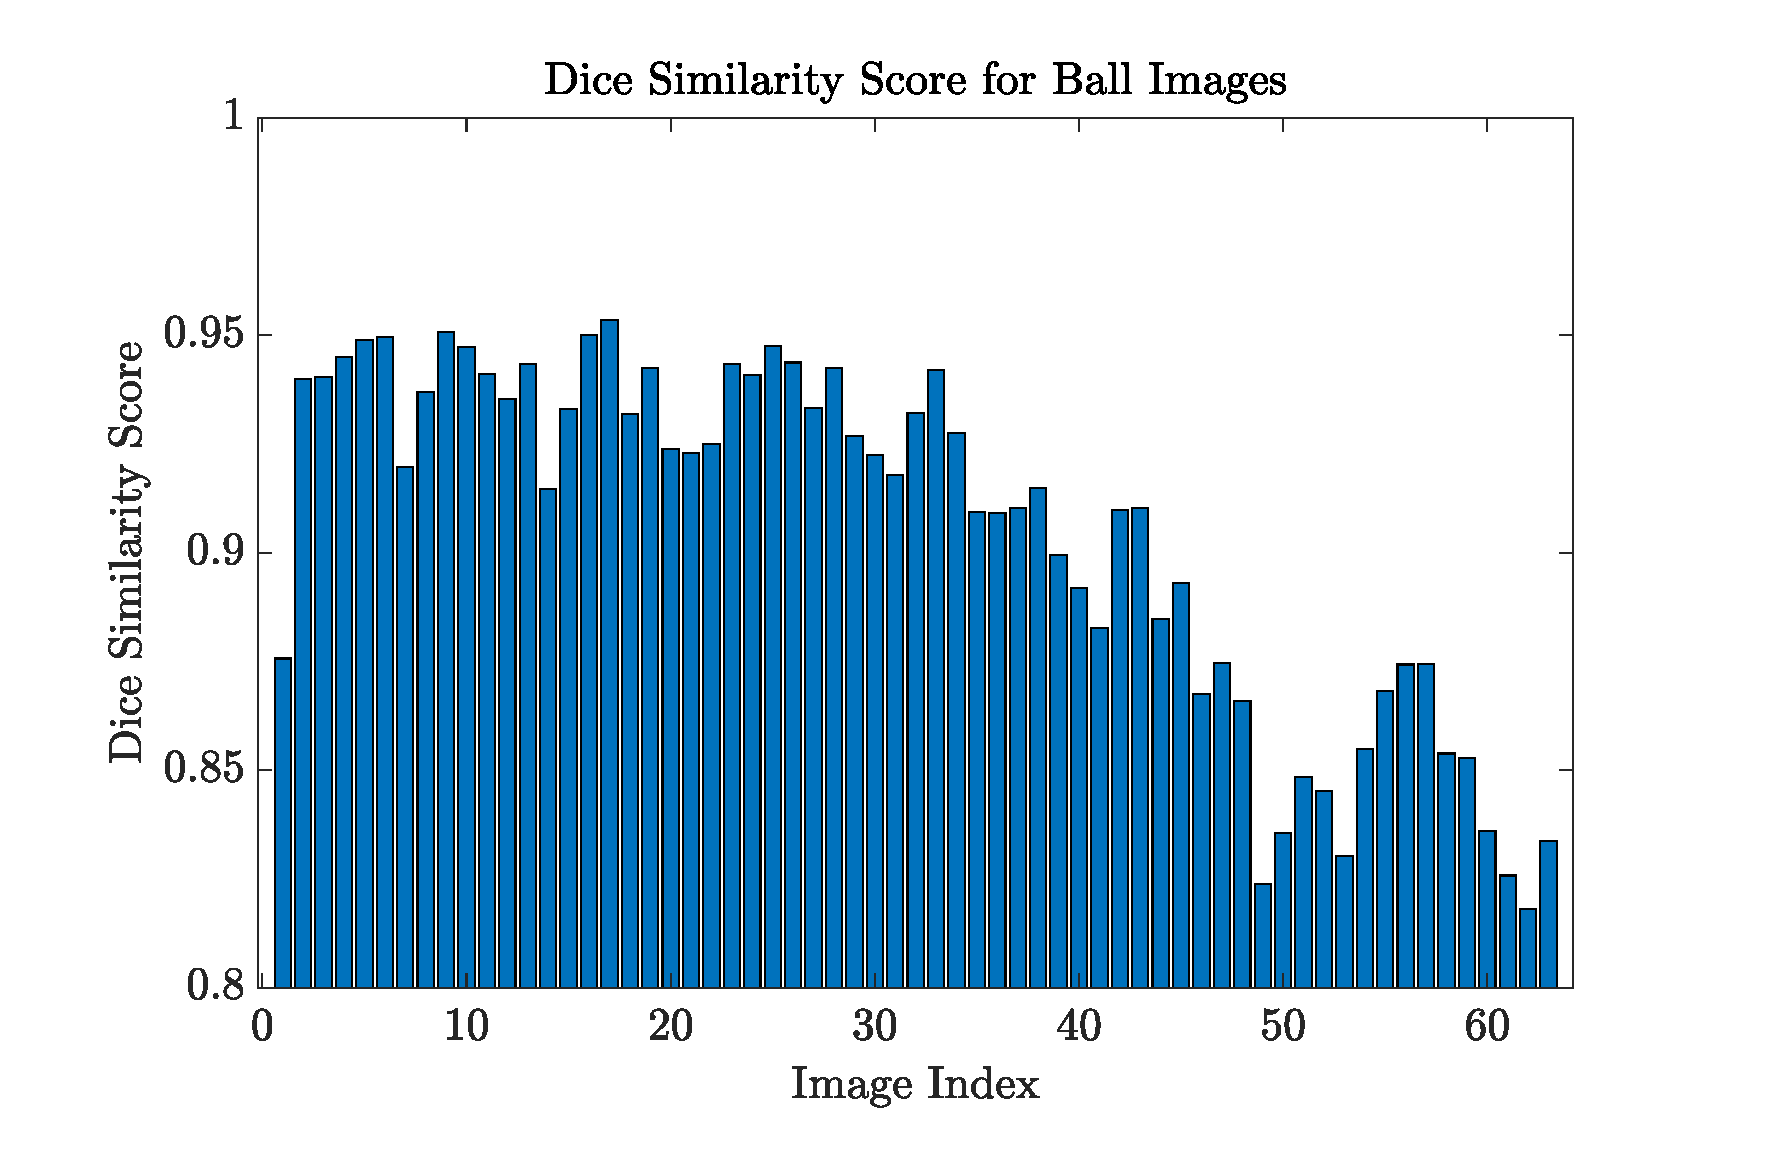
\includegraphics[width=\columnwidth]{figures/DS_bar_graph.pdf}
    \caption{Dice Similarity score for all 63 images\label{fig:DS_bar_graph}}
\end{figure}

\section*{Task 2 | Feature Calculation}
%This part of the assignment will deal with feature extraction, more specifically you will be examining texture and 
%shape features. Using the provided GT ball masks to obtain the corresponding ball patches from original RGB images, 
%carrying out the following tasks.

\subsection*{Task 2.a | Shape features}
%For each of the ball patches, calculate four different shape features discussed in the lectures (solidity, 
%non-compactness, circularity, eccentricity). Plot the distribution of all the four features, per ball type.

For this task, the following shape features were calculated:
\begin{enumerate}
    \item Solidity: The proportion of the pixels in the convex hull that are also in the object.
    \[\text{Solidity} = \frac{\text{Area of the object}}{\text{Area of its convex hull}}\]
    \item Non-compactness: Compactness is the proportion of the region's pixels to all of the bounding box's pixels. So non-compactness is the inverse of this.
    \[\text{Non-compactness} = 1 - \frac{\text{Area of the object}}{\text{Area of bounding box}}\]
    \item Circularity: The roundness of the object.
    \[\text{Circularity} = \frac{4\pi * \text{Area of the object}}{(\text{Perimeter of the object})^2} * \left(1 - \frac{0.5}{{\text{r}}}\right)\]
    Where r = $\frac{\text{Perimeter of the object}}{2\pi} + 0.5$
    \item Eccentricity: The eccentricity is the proportion of the distance between the foci of the ellipse and the length of its major axis. An eccentricity of 0 means its a perfect circle. An eccentricity of 1 means its a line.
    \[\text{Eccentricity} = \frac{\text{Distance between foci of ellipse}}{\text{Length of major axis of ellipse}}\]
\end{enumerate}


\begin{figure}[htbp]
    \captionsetup{singlelinecheck=off}
    \centering
    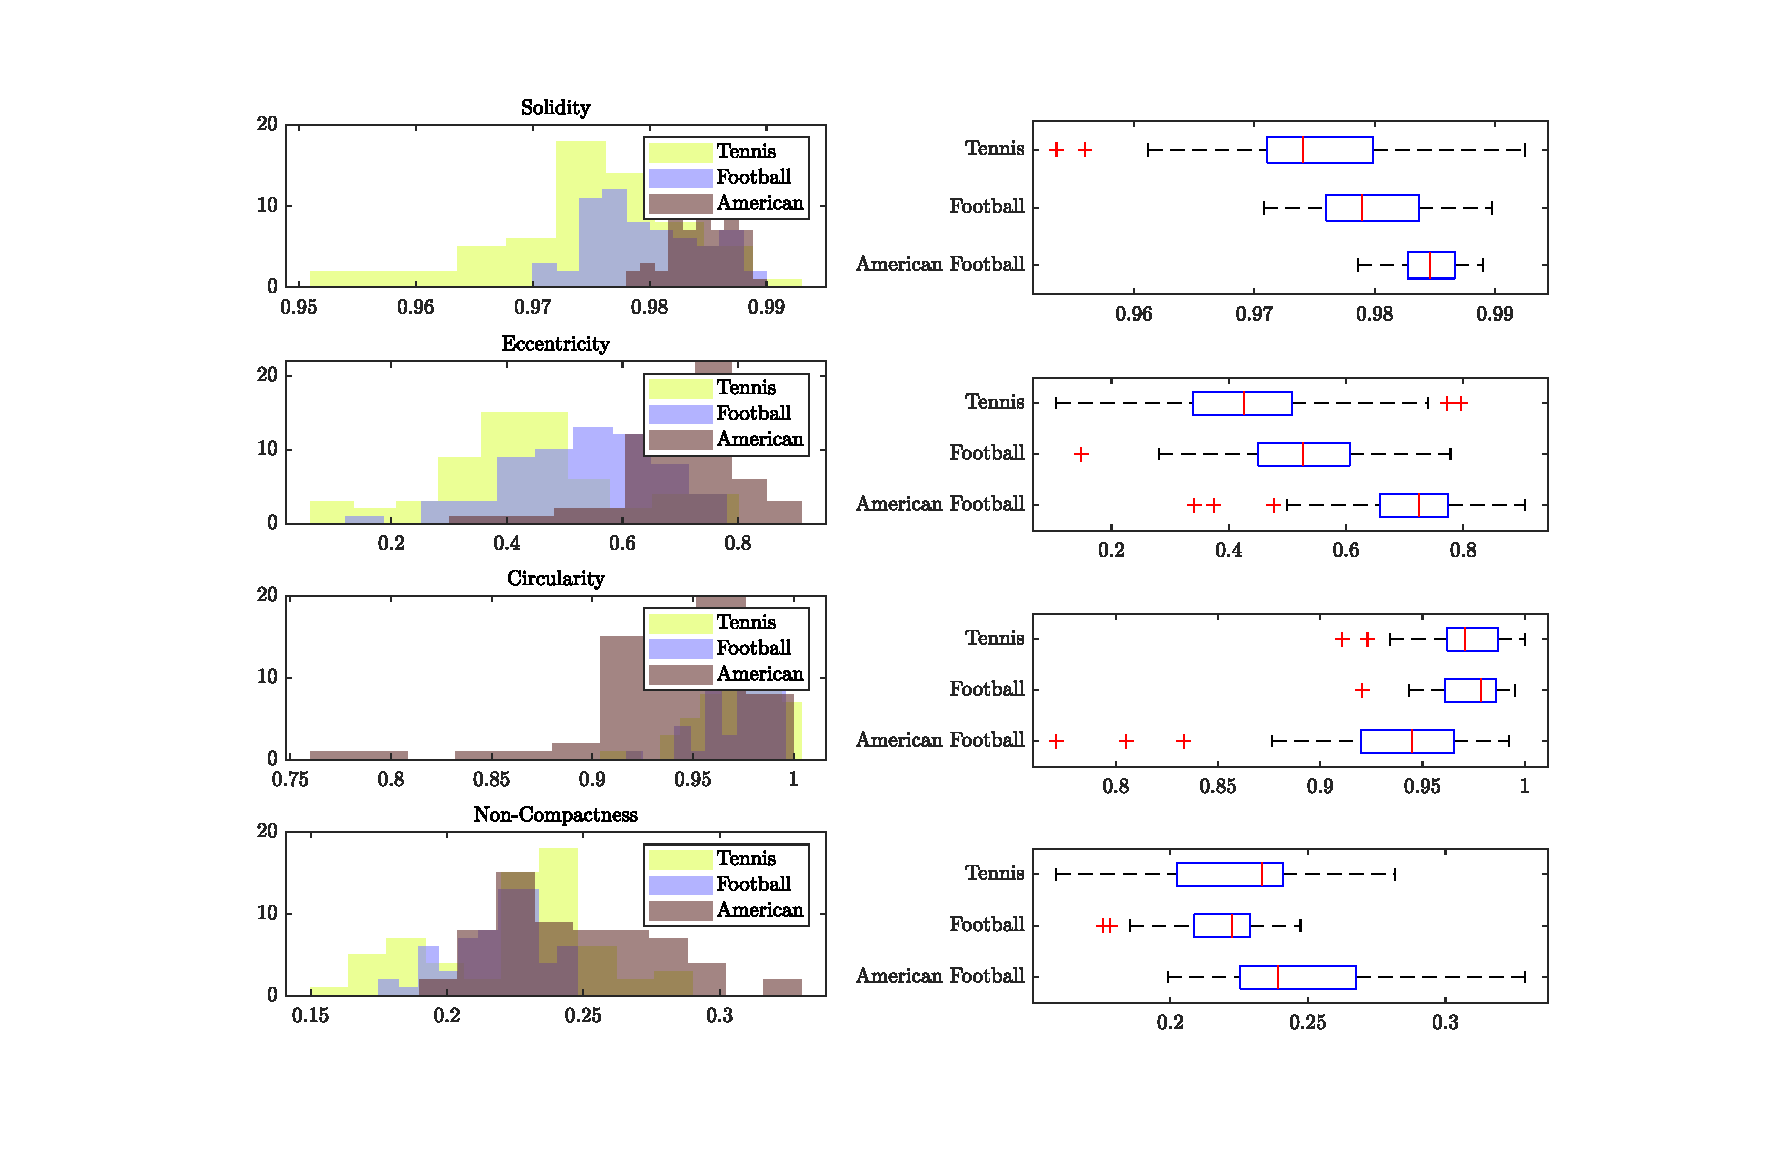
\includegraphics[width=\columnwidth]{figures/shape_feats.pdf}
    \caption[]{Histograms and boxplots showing the Solidity, Non-Compactness, Circularity, and Eccentricity of the three ball types.\\
        Legend: 
        \begin{itemize}
            \item \textcolor{GreenYellow}{yellow}: tennis
            \item \textcolor{CadetBlue}{blue}: football
            \item \textcolor{Tan}{brown}: american football
        \end{itemize}
        \label{fig:shape_feats}
    }
\end{figure}

Figure~\ref{fig:shape_feats} displays histograms and boxplots representing the distribution of four different shape features (solidity, non-compactness, circularity, and eccentricity) for each ball type (tennis, football, and American football).\\
Going through each shape feature one by one. 

There is a lot of overlap between the three ball types for solidity. 
The tennis ball has the lowest median solidity, followed by the football, and then the American football. 
The tennis ball has the highest range of solidity values, followed by the football, and then the american football. 

For Eccentricity, the order of the median values is the same as for solidity but there is less overlap between the three ball types.
This measure seems better at distinguishing the american football from the other two ball types as the american football is not a sphere like the other two balls.

Circularity like eccentricity is better at distinguishing the american football from the other two ball types, with the tennis ball and football having a similar Q1 and Q3 values.
This is also due to the american football not being a sphere like the other two balls.

Finally, non-compactness is the worst at distinguishing between the three ball types as there is a lot of overlap between the three ball types.
The mean of the non-compactness values for each ball lie within 0.025 of each other.

\subsection*{Task 2.b | Texture features}
%Calculate the normalised grey-level co-occurrence matrix in four orientations (0°, 45°, 90°, 135°) for the patches 
%from the three balls, separately for each of the colour channels (red, green, blue). For each orientation, calculate 
%the first three features proposed by Haralick et al. (Angular Second Moment, Contrast, Correlation), and produce 
%per-patch features by calculating the feature average and range across the 4 orientations. Select one feature from 
%each of the colour channels and plot the distribution per ball type.


\begin{figure}[htbp]
    \centering
    \captionsetup{singlelinecheck=off}
    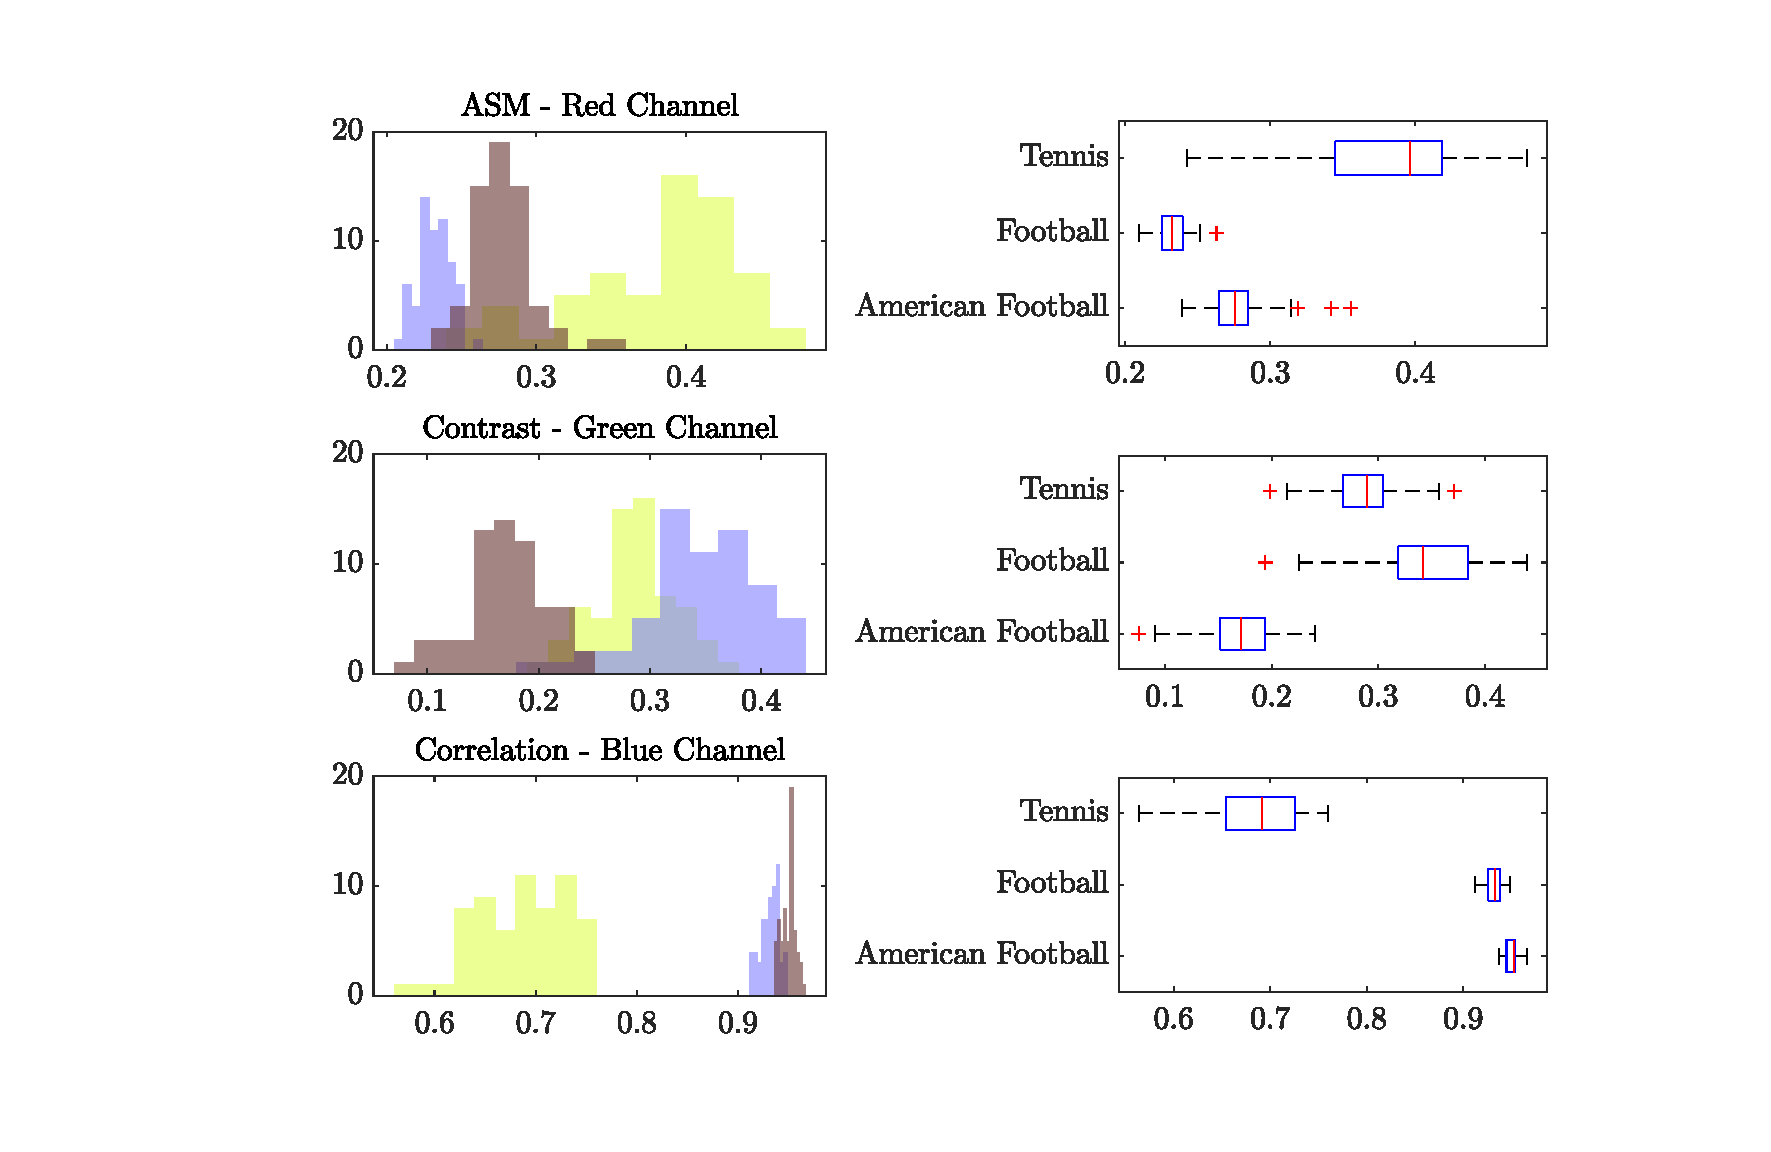
\includegraphics[width=\columnwidth]{figures/averages.pdf}
    \caption[]{Histograms and boxplots showing the average Angular Second Moment, Contrast, and Correlation associated with one colour channel for each ball type.
        Angular Second Moment on the red channel,
        Contrast on the green channel,
        Correlation on the blue channel. Same Legend as Figure~\ref{fig:shape_feats}.
        \label{fig:tex_feats_avgs}
    }
\end{figure}

\begin{figure}[htbp]
    \centering
    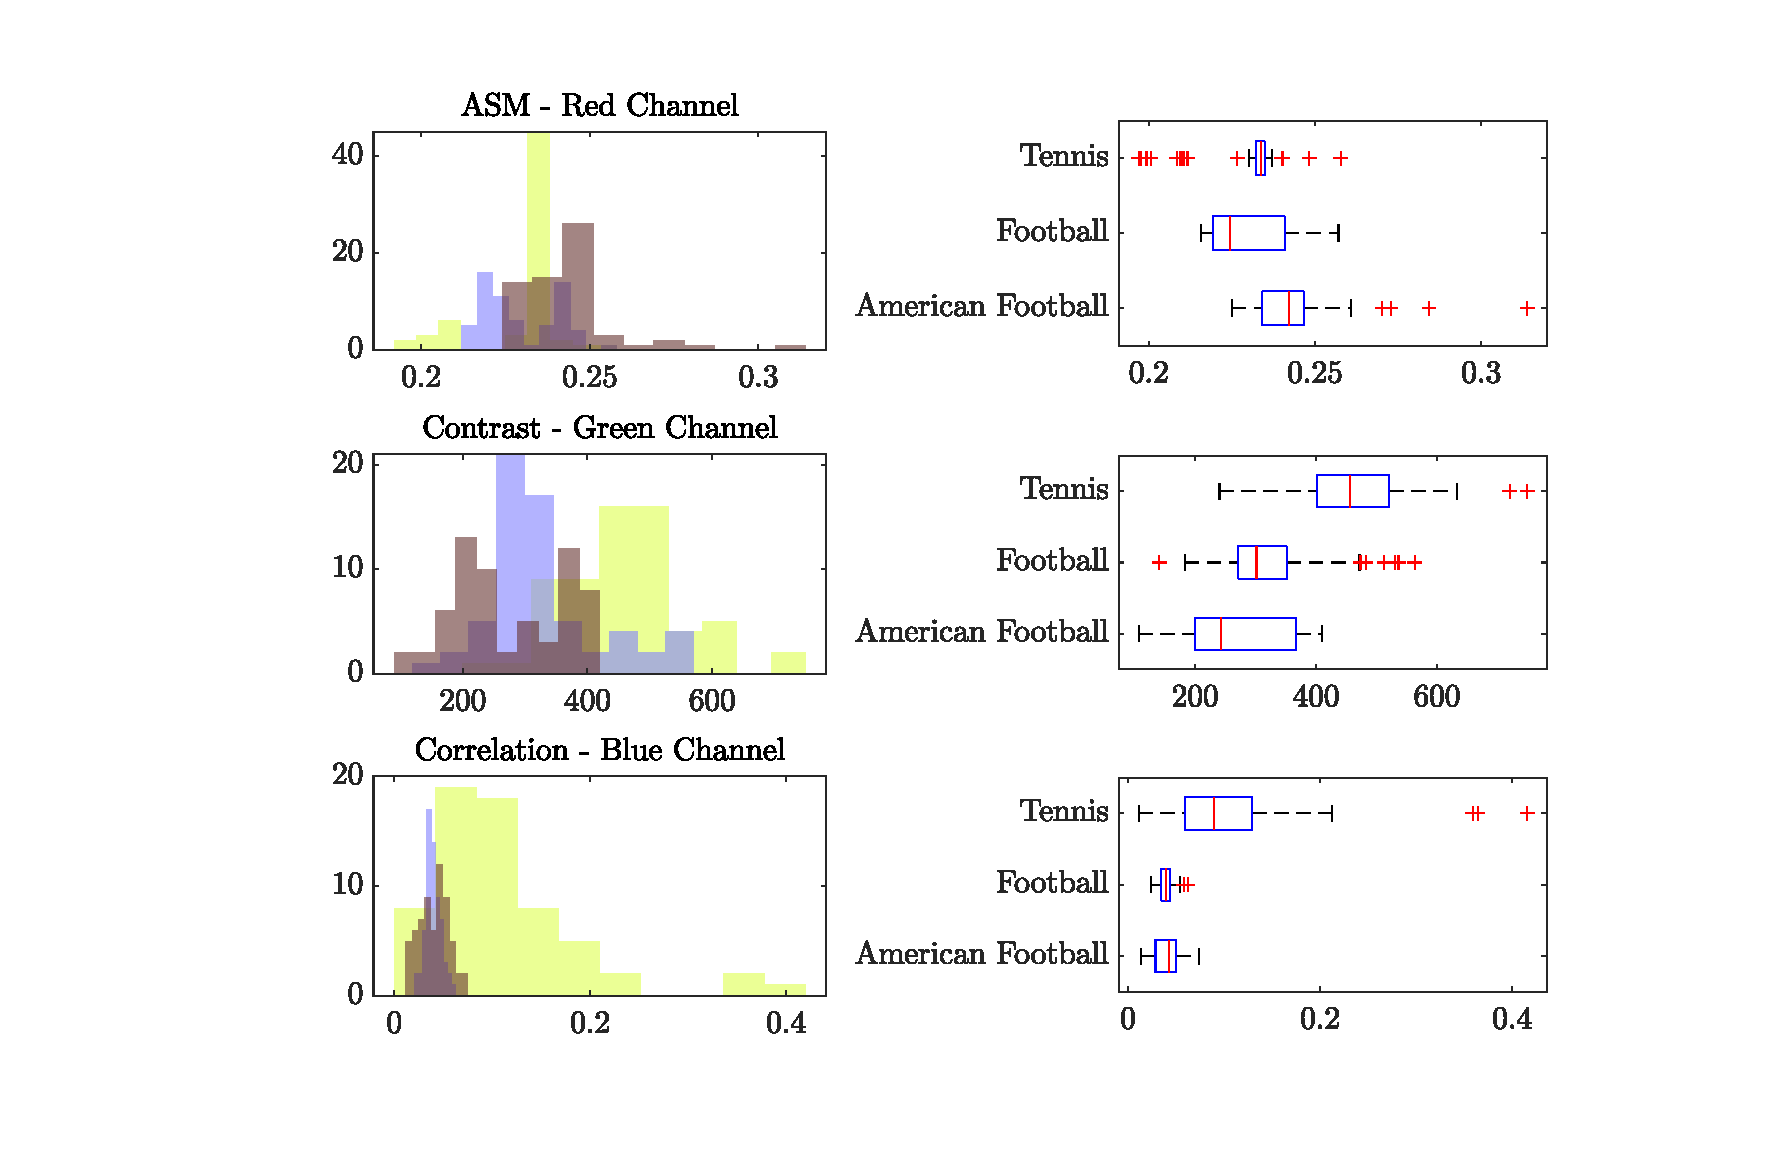
\includegraphics[width=\columnwidth]{figures/ranges.pdf}
    \caption[]{Histograms and boxplots showing the ranges of Angular Second Moment, Contrast, and Correlation associated with one colour channel for each ball type.
        Angular Second Moment on the red channel,
        Contrast on the green channel,
        Correlation on the blue channel. Same Legend as Figure~\ref{fig:shape_feats}.
        \label{fig:tex_feats_ranges}
    }
\end{figure}


\subsection*{Task 2.c | Discriminative information}
%Based on your visualisations in part a) and b), discuss which features appear to be best at differentiating between 
%different ball types. For each ball type, are shape or texture features more informative? Which ball type is the 
%easiest/hardest to distinguish, based on the calculated features? Which other features or types of features would you 
%suggest for the task of differentiating between the different ball types and why?
%Analyse and discuss your findings in the report.



\section*{Task 3 | Object Tracking}
%Download from Blackboard the data files 'x.csv' and 'y.csv', which contain the real coordinates [x,y] of a moving 
%ball, and the files 'na.csv' and 'nb.csv', which contain their noisy version provided by some segmentation and 
%recognition for the football (e.g. frame-to-frame image segmentation of the target). Implement a Kalman filter from 
%scratch (not using any method/class from pre-built libraries) that accepts as input the noisy coordinates [na,nb] and 
%produces as output the estimated coordinates [x*,y*]. For this, you should use a Constant Velocity motion model F with 
%constant time intervals Δt = 0.5 and a Cartesian observation model H.

\subsection*{Task 3.a | Kalman filter tracking}
%You should plot the estimated trajectory of coordinates [x*,y*], together with the real [x,y] and the noisy ones [a,b] 
%for comparison. Discuss how you arrive to the solution.

\begin{figure}[htbp]
    \centering
    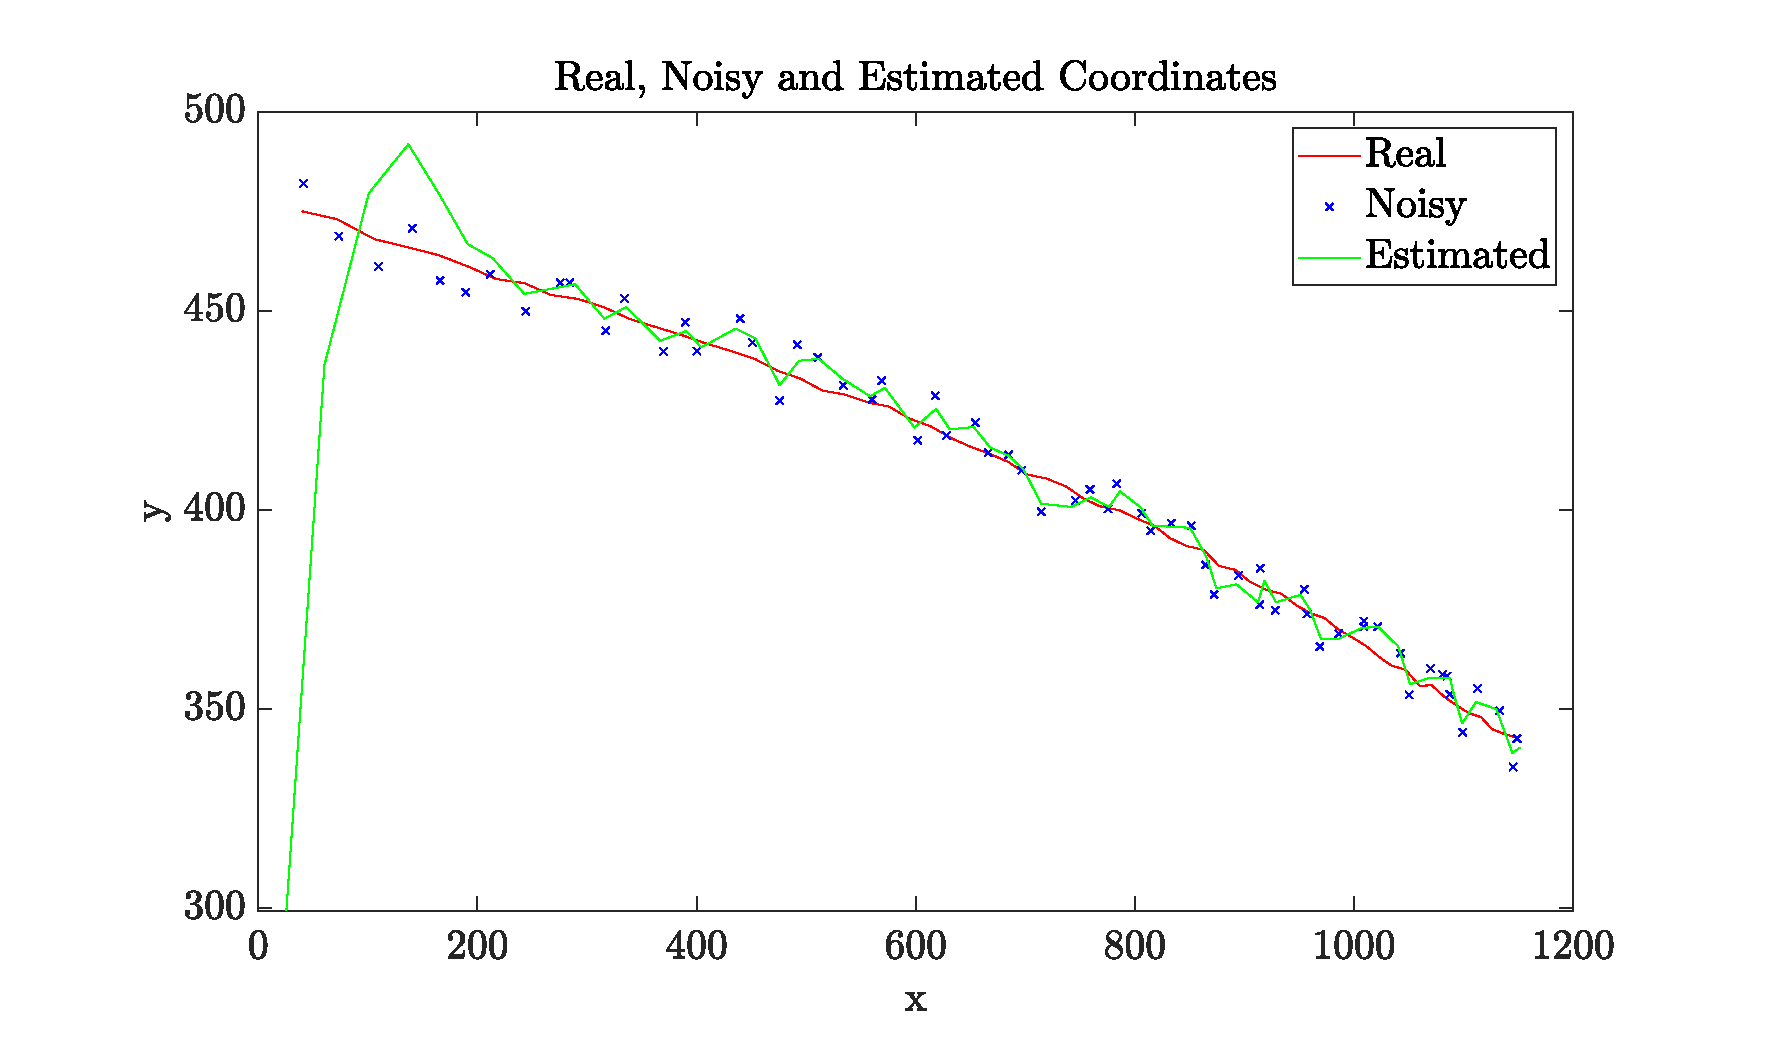
\includegraphics[width=\columnwidth]{figures/kalman.pdf}
    \caption{plot of the estimated trajectory of coordinates $[x_, y_]$, together with the real $[x,y]$ and the noisy $[na, nb]$ for comparison\label{fig:kalman}}
\end{figure}

\subsection*{Task 3.b | Evaluation}
%You should also assess the quality of the tracking by calculating the mean and standard deviation of the Root Mean 
%Squared error (include the mathematical formulas you used for the error calculation in your report). Compare both 
%noisy and estimated coordinates to the ground truth. Adjust the parameters associated with the Kalman filter, justify
% any choices of parameter(s) associated with Kalman Filter that can give you better estimation of the coordinates that
% are closer to the ground truth. Discuss and justify your findings in the report.

\appendix

\begin{figure}[htbp]
    \centering
    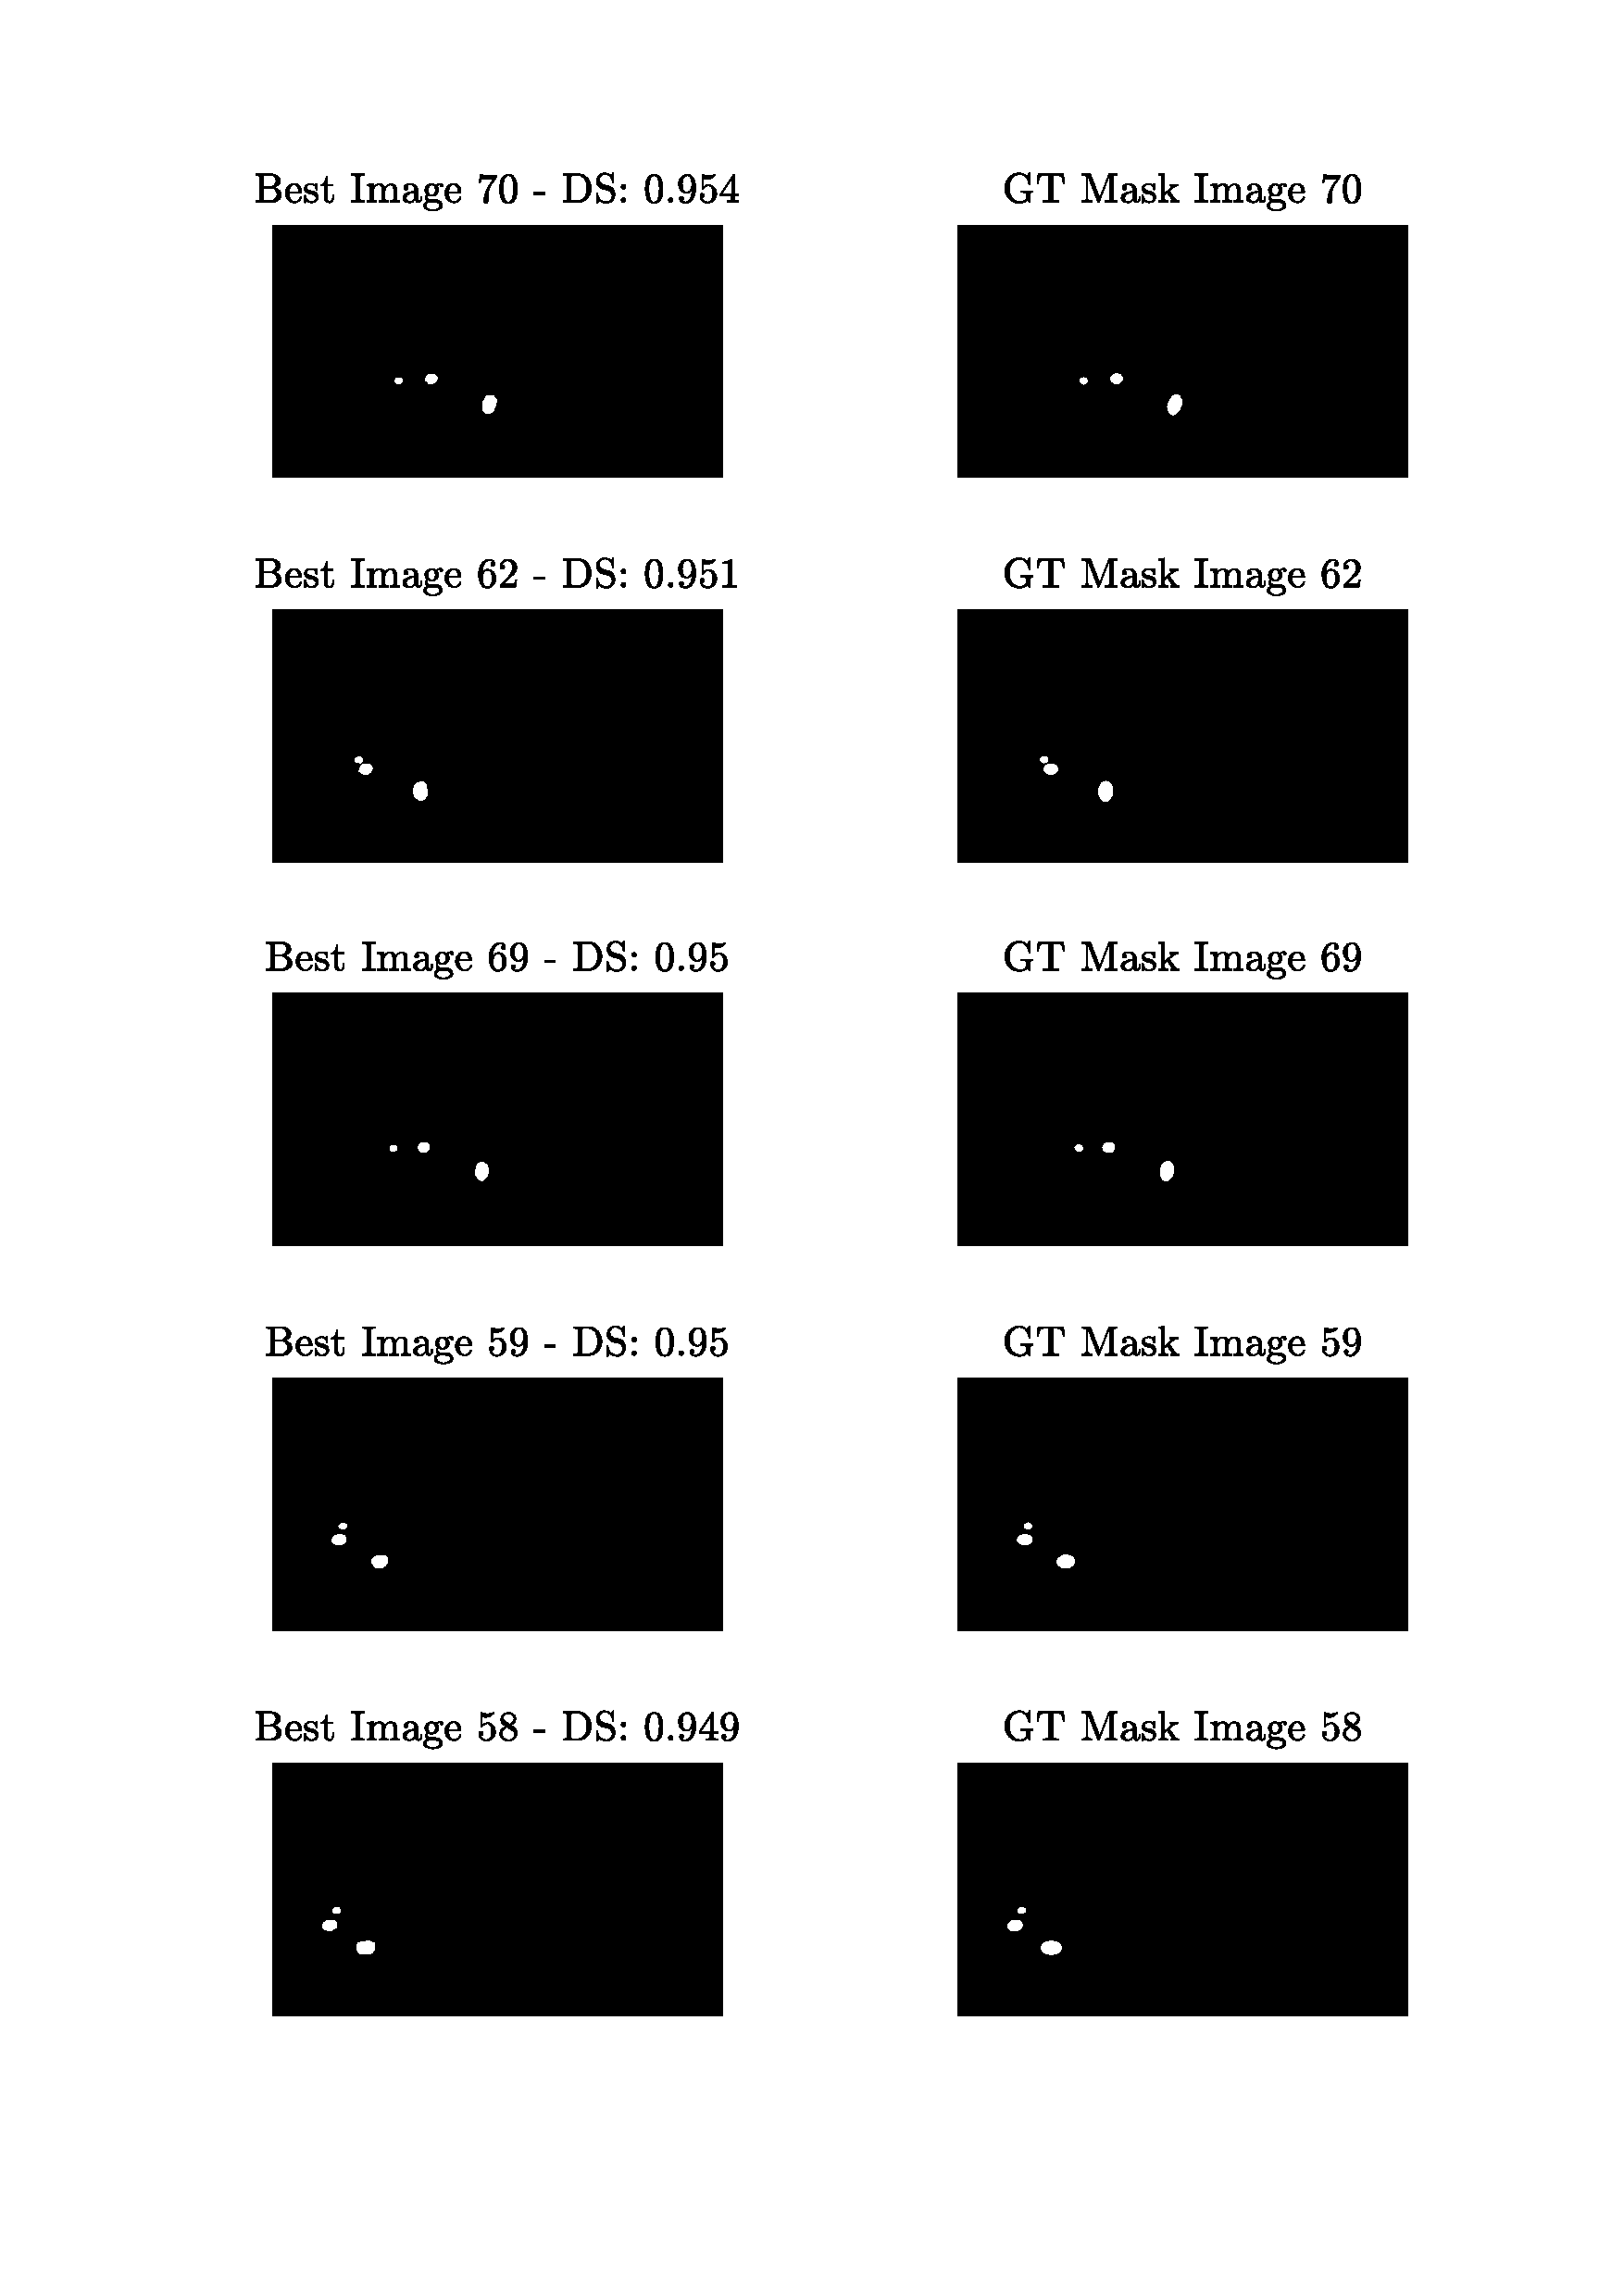
\includegraphics[width=\columnwidth]{figures/best.pdf}
    \caption{Best 5 segmented ball images compared to the ground truth\label{apx:best}}
\end{figure}
\begin{figure}[htbp]
    \centering
    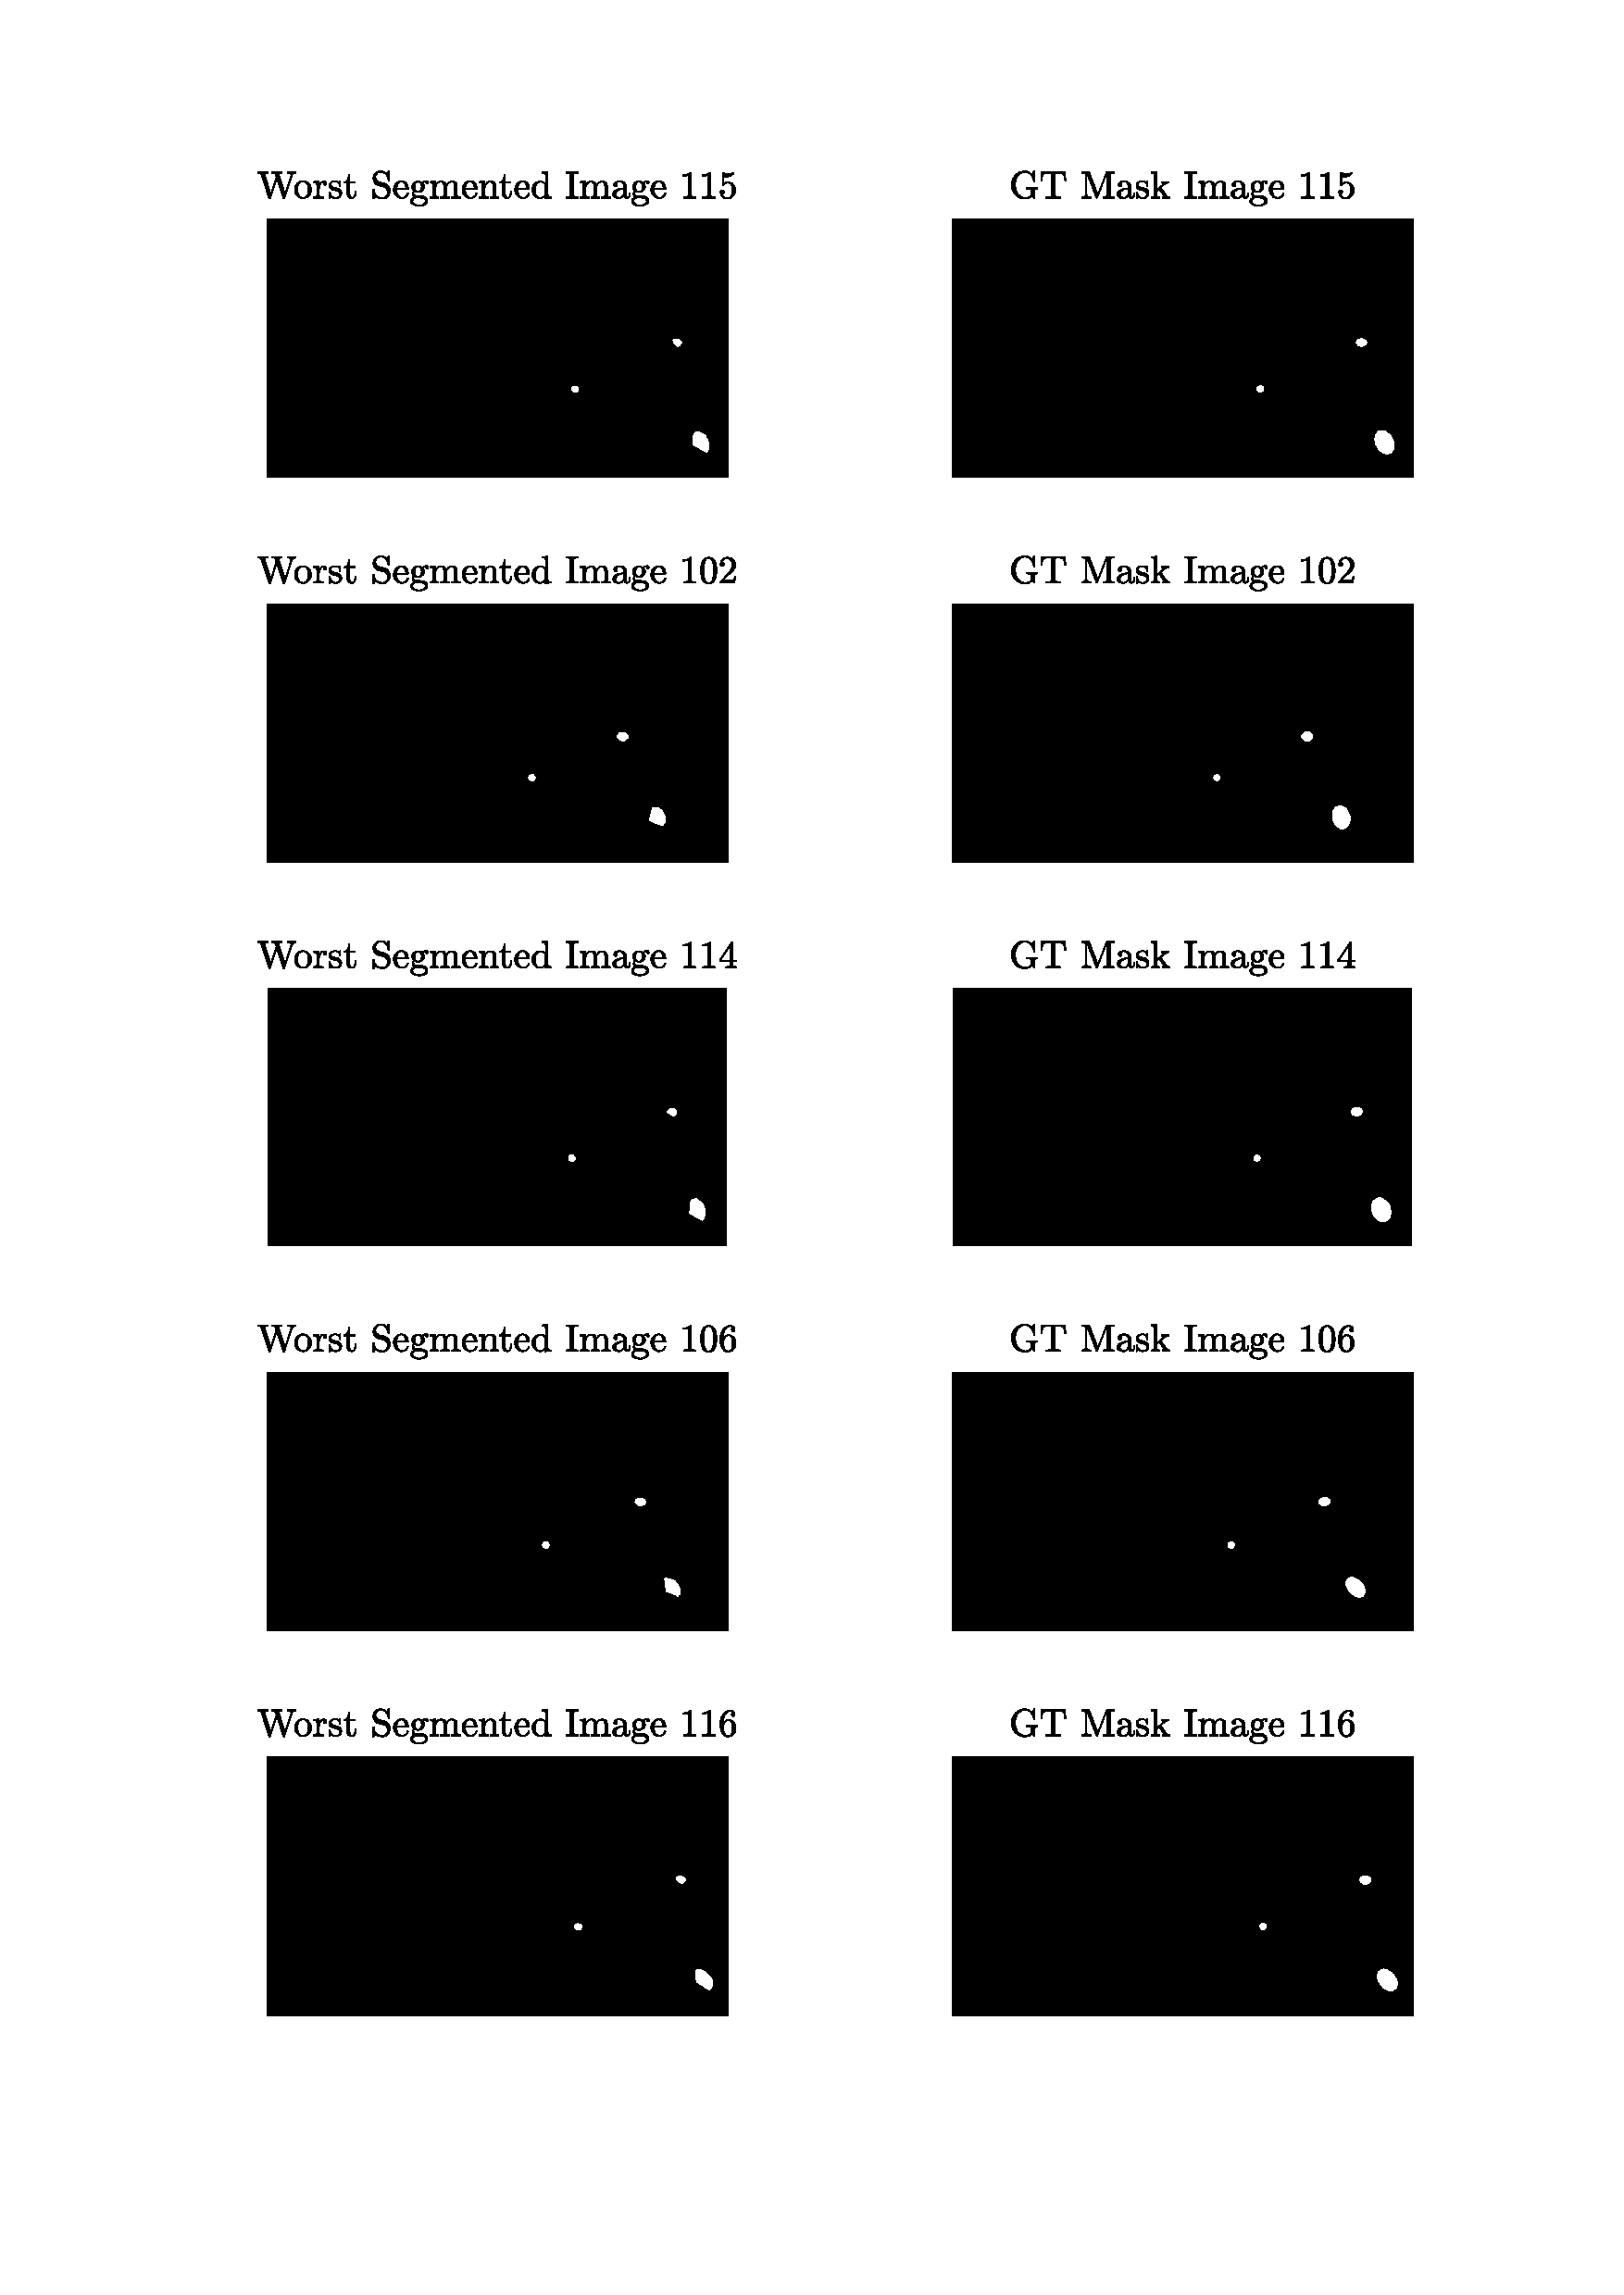
\includegraphics[width=\columnwidth]{figures/worst.pdf}
    \caption{Worst 5 segmented ball images compared to the ground truth\label{apx:worst}}
\end{figure}


\end{document}
